% The five roots z_1, ..., z_5 of a quintic in the complex plane. The two
% red roots z_1, z_2 are smoothly swapped along two non-intersecting paths
% (red arrows) that avoid the other three (blue) roots, so a continuous
% root-selector R is tricked into changing its output.
% Source: book/tex/complex-ana/quintic.tex (section: Step 1).
\documentclass[border=2mm]{standalone}
\usepackage{tikz}
\usetikzlibrary{arrows.meta}
\begin{document}
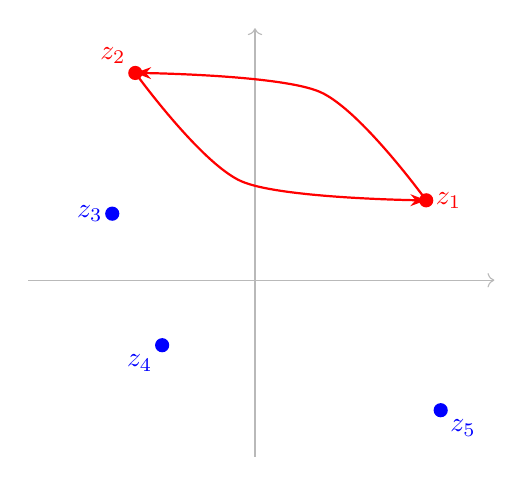
\begin{tikzpicture}[scale=1.6]
  % Complex plane axes.
  \draw[->, gray!55] (-1.8,0) -- (1.9,0);
  \draw[->, gray!55] (0,-1.4) -- (0,2.0);
  % Roots: z_i = mag[i] * dir(dirs[i]).
  % z_1 = 1.5 dir(25),  z_2 = 1.9 dir(120)   (red, being swapped)
  % z_3 = 1.25 dir(155), z_4 = 0.9 dir(215), z_5 = 1.8 dir(325) (blue)
  % Swap paths (red), each a smooth spline through a bulging control point.
  \draw[red, thick, -{Stealth[length=2mm]}]
    plot[smooth] coordinates {(1.359,0.634) (0.517,1.494) (-0.950,1.645)};
  \draw[red, thick, -{Stealth[length=2mm]}]
    plot[smooth] coordinates {(-0.950,1.645) (-0.108,0.785) (1.359,0.634)};
  % Roots and labels.
  \fill[red]  (1.359,0.634)  circle (1.6pt) node[right]      {$z_1$};
  \fill[red]  (-0.950,1.645) circle (1.6pt) node[above left] {$z_2$};
  \fill[blue] (-1.133,0.528) circle (1.6pt) node[left]       {$z_3$};
  \fill[blue] (-0.737,-0.516) circle (1.6pt) node[below left] {$z_4$};
  \fill[blue] (1.474,-1.032) circle (1.6pt) node[below right] {$z_5$};
\end{tikzpicture}
\end{document}
